\documentclass{article}
\usepackage[round]{natbib}

\usepackage{fullpage}
\usepackage{listings}
\usepackage{url}

\usepackage{graphicx}
\usepackage{color}

\lstset{language=Python}

% local definitions
\newcommand{\msprime}[0]{\texttt{msprime}}
\newcommand{\ms}[0]{\texttt{ms}}
\newcommand{\stdpopsim}[0]{\texttt{stdpopsim}}

\newcommand{\aprcomment}[1]{{\textcolor{blue}{APR: #1}}}
\newcommand{\dncomment}[1]{{\textcolor{red}{Dom: #1}}}
\newcommand{\sgcomment}[1]{{\textcolor{red}{SG: #1}}}

\begin{document}

\title{Describing demographic models is hard}
\author{A permutation of (AR, DN, JK, SG)}
\maketitle

\abstract{
Simulation plays a central role in population genomics studies. Recent years
have seen rapid improvements in software efficiency that make it possible to simulate
large genomic regions for many individuals sampled from large numbers of populations.
The increase in complexity of possible demographic models also provides additional ways
that we can get their implementation wrong. Here we describe two errors made in
defining population genetic models using the \msprime\ coalescent simulator that have
found their way in the published record.
We discuss how these errors have affected analyses and suggest recommendations
for software developers and users to reduce the risk of such errors.
}

\section{Introduction}

The \msprime\ coalescent simulator~\citep{kelleher2016efficient,kelleher2020coalescent}
is now quite widely used. The large increases in efficiency over the classical
\ms\ program~\citep{hudson2002generating} make it feasible to simulate large
samples of whole chromosomes for the first time. Another distinct advantage
of \msprime\ is the Python API that is its primary interface, greatly
increasing the flexibility and ease of use over the standard approach of
text-based command line interfaces. In particular, programs like \ms\
required users to specify cryptic command line options to describe demographic
models [JK: maybe include an example ms command line?]. Particularly for
the large models we are using today, these are not comprehensible for humans.
\dncomment{That's a pretty strong statement, might be good to give an example
or describe what it would look like (``specifying the gravel ooa model would take
10K lines of parameter specification''), or just say that its much less intuitive and
so more error prone} \sgcomment{I think it's fine, esp. with JK's suggestions}
The Python API for \msprime\ is a great improvement, allowing the user to
state models in a documented and reproducible manner. [JK: maybe show
the same model as described above in msprime notation?]

Implementing multi-population models of demographic history is still hard and error
prone, however. In this note we discuss two implementation errors that found their way 
in the scientific record. 

We identify two unfortunate design decisions in \msprime's demography API 
that paved the way for these errors, and highlight  




\section{A bad tutorial example}

To illustrate the demography API, \msprime\ included a description of a widely-used
three population Out-of-Africa model~\citep{gutenkunst2009inferring} 
as part of its tutorial documentation. In this model (Fig.~\ref{fig:ooa_stats}A),
Eurasian (CEU and CHB) and African (YRI) populations split from each other in the deep past,
followed by a more recent split of European and Asian populations, with variable rates of
continuous migration between each of the populations. However, the implementation in the
\msprime\ tutorial was incorrect. Namely, at the time of the split between African and Eurasian
populations, migration between those two populations was allowed to continue for all time into the
past. Even though the population split was implemented correctly, the specified demographic model had 
an additional population prior to the earliest split exchanging migrants with the ancestral population 
(Fig.~\ref{fig:ooa_stats}B) but not contributing otherwise to present-day populations.  

Fortunately, the effect of this additional 'ghost' population are subtle. Population sizes and structure since the time of
the split are unaffected, so that differences in expected $F_{ST}$ are negligible between
the correct and incorrect model. However, the presence of the ghost population increases
the effective population size and thus affects the distribution of older $T_{MRCA}$ and the expected 
heterozygosity in each of the three populations by up to $4\%$ (Fig.~\ref{fig:ooa_stats}C-G).

This model was subsequently copied
several times and used in publications [JK: do we want to estimate how
many times it was copied? A quick search on github suggests around 30
times]. \dncomment{I like this as a rough metric, like ``the number of copies
is unknown, but we found x copies on github''}

Such errors could be prevented by improved API design choice.
Currently, to model a population split, the user must use a MassMigration event to move
lineages from one population to another they must then also remember to turn off migration
between those populations at the same time.
The release of \msprime\ 1.0 will introduce a \texttt{PopulationSplit} event, which allows
such models to be described more declaratively.
\dncomment{Strikes me as a bit programmer-centric. Maybe intuitively? Simply?}
\sgcomment{maybe something like "... \texttt{PopulationSplit}  event, which will link the changes in 
the number of populations to changes in demographic parameters such as
migration rates and effective population sizes"  }

\section{A missing parameter}

In another publication using this model~\citep{martin2017human},
a separate error was introduced: the model itself was defined as suggested
in the documentation (using updated parameters~\citep{gravel2011demographic}) and inspected using the \msprime\
debugging tools. After these initial checks were made, however, the simulation
was performed without passing the parameter of demographic events,
so that the three populations remain separated with low levels of migration and
never merge as expected (Fig~\ref{fig:prs}A),
leading to a vast overestimate of the divergence across human populations. 
Whereas the correct model predicts a mean $F_{ST}$ of
$0.05 - 0.10$ across the three population, the simulated model generated $F_{ST}$
ranging between $0.3 - 0.6$, depending on the populations considered.

This simulation was performed to assess the
transferability of polygenic risk scores across human populations, in particular to
explore how human demographic history and population structure affects our ability
to predict genetic risk in populations of different ancestry than the originally studied
population. 
The excess divergence exaggerates the role that demography plays in limiting the transferability
of genetic risk scores across populations. The resulting publication has been influential in the discussion of
health inequalities and genomics, with over 350 citations since 2017.
We note that while difficulties in transferability remain in the corrected model
(Fig.~\ref{fig:prs}), risk prediction in each population is significantly improved
when using the correct demographic model (compare to Fig.~5 in~\citet{martin2017human}.

These errors suggests three lessons.
First, the design of user interface and API for scientific software matters,
and many bugs can be prevented by using more intuitive 
interfaces. Whereas the original msprime required the user to pass
three separate parameters to specify a demographic model, \msprime\ 1.0
 introduces a Demography class, which wraps these three parameters.
Thus, instead of writing
\begin{lstlisting}[frame=single]
dbg = msprime.DemographyDebugger(
  population_configurations=population_configurations,
  migration_matrix=migration_matrix,
  demographic_events=demographic_events)
dbg.print_history()
ts = msprime.simulate(
  population_configurations=population_configurations,
  migration_matrix=migration_matrix,
  demographic_events=demographic_events),
\end{lstlisting}
with the error-inducing need to re-enter parameter information,  
we would now write
\begin{lstlisting}[frame=single]
demography = msprime.Demography(
  population_configurations=population_configurations,
  migration_matrix=migration_matrix,
  demographic_events=demographic_events)
dbg = demography.debug()
dbg.print_history()
ts = msprime.simulate(demography=demography)
\end{lstlisting}

Second, testing of the final simulated data is important. This can be challenging,
because the amount of simulated data can be large. However, recent progress in
computing summary statistics from tree sequence data can make this
easier~\citep{ralph2020efficiently}.
Even if the entire simulation data cannot be easily evaluated, subsets of the data
can be examined to identify large errors.

Third, open data analysis pipelines are necessary for the self-correcting nature of science.
This subtle error of large effect was only discovered through our own re-use of
the simulation pipeline developed in~\citep{martin2017human} to pursue
additional analyses on a similar topic. We identified the bug by tracing down an unexpected
result in our analysis. This error could not have been found and corrected without the open
publication of the entire analysis pipeline from the original study.

\section{Conclusions}

The implementation of complex demographic models is error prone, and such errors can 
have a large impact on downstream analysis and interpretation. 
Recognition of these difficulties drove efforts to standardize and peer-review demographic model
implementation in \stdpopsim~\citep{adrion2019community}, with quality-controlled
models and simulation resources for a growing number of commonly studied species. 

The first bug discussed in this note was indeed identified through a peer-review effort of the 
model implementation,  and it would have been unlikely to be identified by inspection of the 
resulting data. The second bug would have been comparably easy to identify by inspection of the data, 
but the missing parameter was easy to overlook. 

We therefore recommend the following steps to ensure more robust simulations.
First, we recommend that demographic models used in publications 
are systematically verified by a second pair of eyes in code review. If the implementation is complex enough
that code review is impractical, the risk that bugs are introduced is extremely high and the software 
interface likely needs design improvements. 

Second, we recommend basic statistical verification of all simulated data. If simulations are so large that
statistical validation is burdensome, subsets of the simulated data can be analyzed. 
\sgcomment{Here again, software design can help by providing functions to compute 
basic statistics of genetic diversity. [...]}. Such tests would have caught the error in~\citet{martin2017human}.


Third, and most importantly, openness is essential. We only know about these errors because of open code and
open source development processes. By making their entire pipeline available, \citet{martin2017human} not only 
enabled other research teams to build upon their findings, but they also enlisted the entire community to review their code. 

There must be many, many more mistakes out there, and we need both pre- and post-publication vigilance from 
users and developers to ensure the soundness of the large body of simulation-based analyses. 


\section{Methods}

\begin{itemize}
\item Figure 1 used plotting routine from the \texttt{demography} package (\url{https://github.com/apragsdale/demography}),
allele frequency spectrum computed using \texttt{moments}~\citep{jouganous2017inferring}, and LD curves
computed using \texttt{moments.LD}~\citep{ragsdale2019models}. $F_{ST}$ and other statistics computed
from the expected AFS.
\item Figure 2 used the original pipeline from \url{https://github.com/armartin/ancestry_pipeline/blob/master/simulate_prs.py},
and was rerun using corrected parameters, with code available at \url{https://github.com/apragsdale/PRS}
\end{itemize}

\bibliographystyle{plainnat}
\bibliography{paper}

\pagebreak

\begin{figure}[ht]
\begin{center}
\makebox[\textwidth][c]{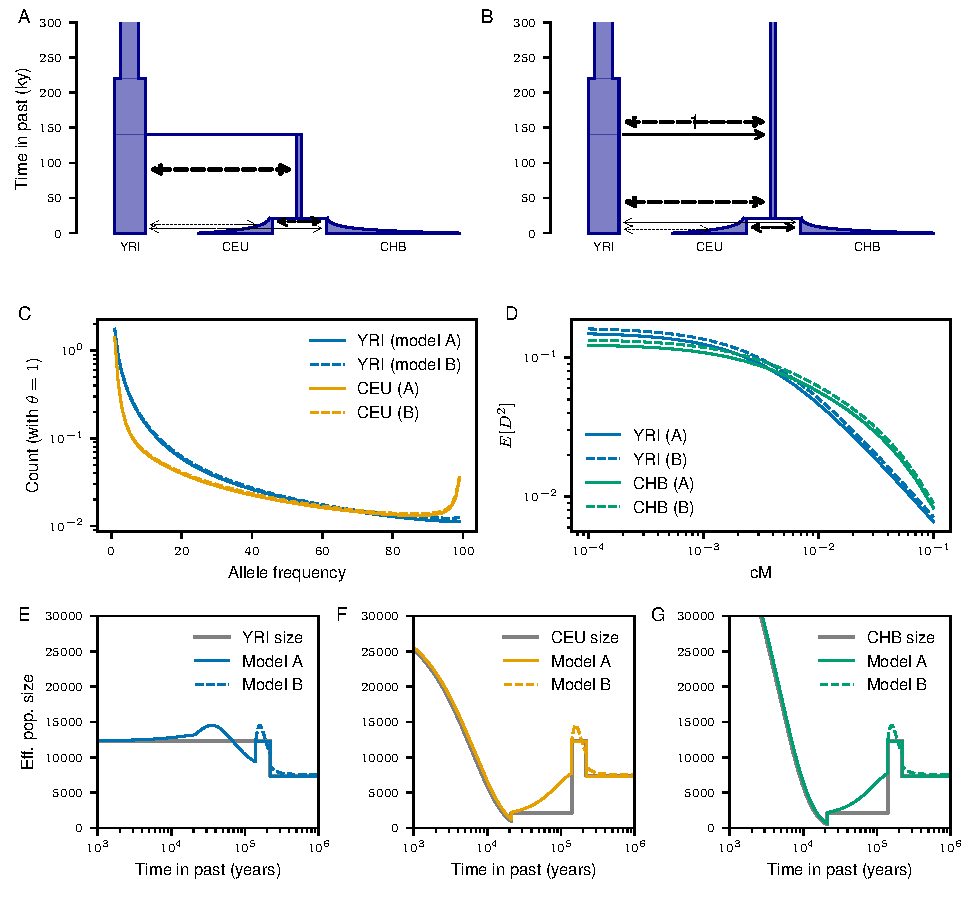
\includegraphics{figures/ooa_expected_stats.pdf}}
\caption{\textbf{Expected diversity statistics under the \citet{gutenkunst2009inferring} model}.
    \textbf{(A)} The correctly implemented model.
    \textbf{(B)} The incorrectly implemented model from the \msprime\ tutorial, with migration continuing
    into the past.
    \textbf{(C)} Marginal allele frequency spectra under the two models. Heterozygosity in the incorrect model
    is inflated by $~3.5\%$, though the general shape of the distributions are qualitatively similar.
    \textbf{(D)} Similarly, the increased heterozygosity leads to excess $D^2$, though the LD-decay is
    qualitatively similar between models.
    \textbf{(E-G)} True size history for each population plotted against the expected size history from
    the expected inverse coalescence rates.
    \sgcomment{Not sure what the 1 in Figure 1b means. I would put the mass migration arrow in blue. }
}
\label{fig:ooa_stats}
\end{center}
\end{figure}

\begin{figure}[ht]
\begin{center}
\makebox[\textwidth][c]{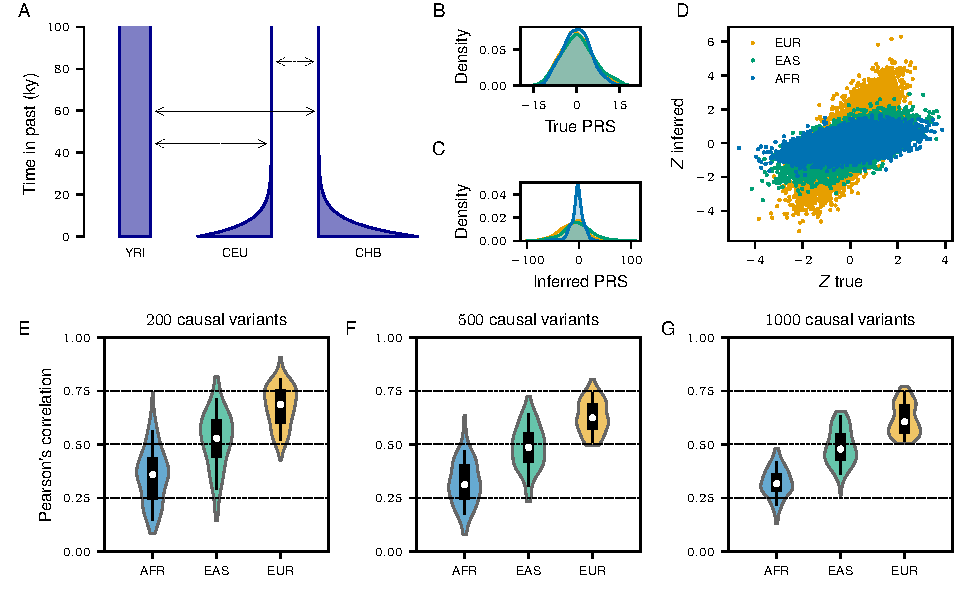
\includegraphics{figures/prs_fig.pdf}}
\caption{\textbf{The transferability of PRS under neutrality}.
    \textbf{(A)} In~\citet{martin2017human}, the simulated demographic model did not apply demographic
    events in the past, so continental populations were simulated as isolated with low levels of migration
    for all time. The intended model is shown in Figure \ref{fig:ooa_stats}.
    \textbf{(B-G)} We repeated the simulation experiment in~\cite{martin2017human} using the correct
    demographic model and found that risk prediction was greatly improved over what was originally
    reported in all three populations.
    \aprcomment{directly compare to figure 5 in the original paper} \sgcomment{If we }
    \aprcomment{to do: fill in caption}
}
\label{fig:prs}
\end{center}
\end{figure}


\end{document}
